% =============================================================================
% Compile parameters
% =============================================================================

\documentclass[12pt, russian]{extarticle}
\usepackage[utf8]{inputenc}
\usepackage[T2A]{fontenc}
\usepackage{fontspec}
\defaultfontfeatures{Ligatures={TeX},Renderer=Basic}
\setmainfont[Ligatures={TeX,Historic}]{Times New Roman}
\usepackage[a4paper,
left=25mm,
right=15mm,
top=20mm,
bottom=20mm]{geometry}
\usepackage[linktoc=all]{hyperref}
\usepackage{titlesec}
\titlelabel{\thetitle.\quad}
\usepackage{tocloft}

% Remove \bfseries from section titles in ToC
\renewcommand{\cftsecfont}{}
% Remove \bfseries from section titles' page in ToC
\renewcommand{\cftsecpagefont}{}
\renewcommand{\cftsecaftersnum}{.}
\usepackage{titlesec}

% Change font size for types
\titleformat*{\section}{\large\bfseries}
\titleformat*{\subsection}{\large\bfseries}
\titleformat*{\subsubsection}{\large\bfseries}

\setlength{\parindent}{1.25cm}
\setlength{\parskip}{0.4cm}
\font\subtitlefont=cmr12 at 12pt
\font\titlefont=cmr12 at 24pt
\usepackage{color}
\usepackage{mathtools}
\usepackage{listings}
\usepackage{graphicx}
\usepackage{tocloft}
\usepackage{indentfirst}
\usepackage{enumitem}
\usepackage{graphicx}
\usepackage{subcaption}
\usepackage{babel}
\usepackage{setspace}
\renewcommand{\contentsname}{}
\renewcommand{\cftsecleader}{\cftdotfill{\cftdotsep}}
\graphicspath{ {./resources/} }

\usepackage{listings}
\definecolor{dkgreen}{rgb}{0,0.6,0}
\definecolor{gray}{rgb}{0.5,0.5,0.5}
\definecolor{mauve}{rgb}{0.58,0,0.82}
\lstset{
    language=Python,
    basicstyle=\ttfamily\small,
    keywordstyle=\color{blue},
    commentstyle=\color{dkgreen},
    stringstyle=\color{mauve},
    stepnumber=1,
    breaklines=true,
    breakatwhitespace=true,
    tabsize=4,
    captionpos=tl,
}

% =============================================================================
% End of compile parameters
% =============================================================================

\title{}
\author{}
\date{}

\begin{document}

% =============================================================================
% Global titlepage
% =============================================================================

\begin{titlepage}

    \begin{center}
        МИНИСТЕРСТВО НАУКИ И ВЫСШЕГО ОБРАЗОВАНИЯ РОССИЙСКОЙ ФЕДЕРАЦИИ \\
        Федеральное государственное автономное образовательное учреждение \\
        высшего образования \\
        \textbf{
            «Национальный исследовательский \\
            Нижегородский государственный университет им. Н.И. Лобачевского»\\ (ННГУ)
        }
    \bigbreak

    \vspace{2em}
        \textbf{
            Институт информационных технологий, математики и механики
            \bigbreak
            Кафедра математического обеспечения и суперкомпьютерных технологий
        }

        Направление подготовки: «Программная инженерия» \\
        Профиль подготовки: «Разработка программно-информационных систем»

        \bigbreak
        \bigbreak
        \bigbreak

        \textbf{ВЫПУСКНАЯ КВАЛИФИКАЦИОННАЯ РАБОТА БАКАЛАВРА}
        \bigbreak

        на тему \\
        {\bfseries ``Разработка программно-аппаратного комплекса для мониторинга показателей сердца
        человека''}
    \end{center}

    \vspace{5em}

    \begin{flushright}
        {\bfseries Выполнил:} студент группы \\ 382008-1 Булгаков Даниил Эдуардович\\
        \hfill Подпись \hspace{5em} \newline \\
        {\bfseries Научный руководитель:} \\доцент кафедры МОСТ, к.т.н., \\ Борисов Николай Анатольевич \\
        \hfill Подпись \hspace{5em} \newline \\
    \end{flushright}


    \vspace{\fill}

    \begin{center}
        Нижний Новгород\\2024
    \end{center}

\end{titlepage}

% =============================================================================
% Main content
% =============================================================================

% ========== Set global spacing ==========
\begin{spacing}{1.5}

% ========== Table of content ==========
\tableofcontents
\thispagestyle{empty}
\newpage

% Params to make the following text start with
% its page number
\pagestyle{plain}
\setcounter{page}{3}

% ========== Introduction ==========
\section{Введение}

Последние несколько лет наблюдается значительный рост числа заболеваний сердечно-сосудистой системы, что делает наблюдение за состоянием сердца важной задачей в области медицины. Одним из наиболее распространенных методов диагностики и мониторинга сердечной активности является электрокардиография (ЭКГ). ЭКГ представляет собой графическую запись электрической активности сердца, которая позволяет выявлять различные аномалии, такие как аритмии, ишемия, инфаркты и другие патологии. Данный метод широко применяется благодаря своей информативности, неинвазивности и доступности.

Несмотря на высокую эффективность традиционных стационарных систем ЭКГ, их применение ограничено рамками медицинских учреждений. Пациенты, особенно страдающие хроническими заболеваниями, нуждаются в постоянном мониторинге сердечной активности, что представляет собой значительную проблему в условиях стационара. В связи с этим, актуальной становится разработка портативных систем для непрерывного мониторинга сердечной деятельности в повседневной жизни.

Целью данной дипломной работы является создание программно-аппаратного комплекса для мониторинга показателей сердца человека. Комплекс включает модуль для регистрации ЭКГ, приложение для передачи данных с модуля на сервер, а также системы сбора, анализа и хранения данных.

% ========== Task definition ==========
\newpage
\section{Описание предметной области}

\subsection{Электрокардиография}

Электрокардиография (ЭКГ) — это метод регистрации и анализа электрических полей, возникающих в процессе работы сердца. Этот метод является сравнительно недорогим, но чрезвычайно ценным инструментом для электрофизиологической диагностики в кардиологии.

\subsection{Электроды}

Электрод — это устройство, предназначенное для проведения электрического тока между телом пациента и электронным прибором. В контексте электрокардиографии (ЭКГ), электроды используются для регистрации электрической активности сердца. Они преобразуют биопотенциалы, возникающие при работе сердца, в электрические сигналы, которые затем обрабатываются и анализируются для диагностики и мониторинга сердечной деятельности.

Электроды играют ключевую роль в обеспечении точности и надежности измерений ЭКГ. Различные типы электродов обладают специфическими характеристиками, которые могут влиять на качество и стабильность записываемых сигналов. Для выбора подходящих типов электродов необходимо основываться на частоте использования, расположения на теле, а также требований к качеству считывания сигнала.

\par \noindent \textbf{Виды электродов:}

\begin{enumerate}
    \item \textbf{Гелевые (мокрые) электроды:} \\
        Покрыты электропроводящим гелем, который улучшает контакт с кожей и снижает электрическое сопротивление.
    \item \textbf{Текстильные электроды:} \\
        Изготавливаются из проводящих текстильных материалов и могут быть интегрированы в одежду.
    \item \textbf{Сухие электроды:} \\
        Изготавливаются из проводящих материалов, таких как металлы или углеродные композиции, и не требуют использования геля.
\end{enumerate}

Для наглядного сравнения была добавлена таблица с преимуществами и недостатками каждого типа электродов (Таблица 1.).

\begin{table}[h!]
    \centering
    \begin{tabular}{| p{5cm} | p{5cm} | p{5cm} |}
    \hline
    \textbf{Тип электрода} & \textbf{Преимущества} & \textbf{Недостатки} \\
    \hline
    \textbf{Гелевые (мокрые) электроды} & Высокая точность и качество сигнала & Ограниченный срок использования из-за высыхания геля, возможное раздражение кожи \\
    \hline
    \textbf{Текстильные электроды} & Удобство и гибкость использования & Менее стабильный контакт с кожей, снижение качества сигнала при движении \\
    \hline
    \textbf{Сухие электроды} & Отсутствие необходимости в геле, сниженный риск раздражения кожи, устойчивость к высыханию, возможность многократного использования & Возможное повышение сопротивления контакта, что может снижать качество сигнала \\
    \hline
    \end{tabular}
    \caption{Преимущества и недостатки различных типов электродов}
    \label{table:electrodes}
    \end{table}

В условиях постоянного использования устройства, как в движении, так и в покое, наиболее оптимальный вариантом являются сухие электроды, которые не требуют нанесения геля при каждом использовании и не теряют качество сигнала при физической активности.

\subsection{Отведения}

Отведения - это способ размещения электродов на теле пациента для получения различных проекций электрической активности сердца. Каждый тип отведения обеспечивает уникальную перспективу наблюдения за электрическими импульсами сердца, что позволяет более детально анализировать работу сердечной мышцы и выявлять различные патологии. 

\noindent Существует несколько стандартных систем отведений:

\begin{itemize}
    \item Стандартные отведения
    \item Усиленные отведения
    \item Грудные отведения
\end{itemize}

\subsubsection{Стандартные отведения}

Стандартные отведения регистрируют разность потенциалов между конечностями человека. Для получения данного типа отведений требуется три электрода: положительный, отрицательный и заземление. Так, правая и левая пара электродов руки образуют первое стандартное отведение - I, электроды правой руки и левой ноги – второе - II, третье отведение III - левая рука и левая нога. Третий электрод используется как заземление (Рис. 1).

\begin{figure}[htbp]
\centering
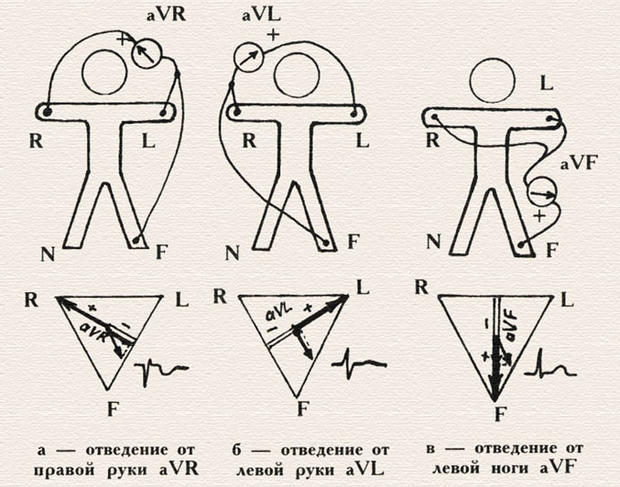
\includegraphics[scale=0.44]{resources/отведения экг.jpg}
\caption{Стандартные отведения.}
\end{figure}

Тогда для получения кардиограммы достаточно вычислить разность потенциалов между указанными сигналами.

\begin{center}
\begin{tabular}{|l|l|}
\hline
\textbf{Отведение}      & \textbf{Вычисление} \\ \hline
\textbf{1-ое отведение} & LA-RA               \\ \hline
\textbf{2-ое отведение} & LL-RA               \\ \hline
\textbf{3-е отведение}  & LL-LA               \\ \hline
\end{tabular} \bigbreak
LA - левая рука, RA - правая рука, LL - левая нога.
\end{center}

Нетрудно заметить, что в случае, когда нам требуется получить значения сразу по трем отведениям, то аппаратно потребуется считывать только два из них, так как третье можно вычислить путем сложения/вычитание двух других, к примеру:

\begin{center}
    1-ое отведение + 3-е отведение = 2-е отведение
\end{center}

Данные отведения позволяют регистрировать следующие типы заболеваний: 

\begin{itemize}
    \item Ишемия миокарда (недостаточное поступление кислорода в сердечную мышцу). Это может проявляться в виде изменений в зубцах ST и T, а также снижения амплитуды зубцов.
    \item Аритмии, такие как фибрилляция предсердий или желудочковые экстрасистолы. Это может проявляться в виде изменений в ритме и частоте сердечных сокращений, а также в форме зубцов на ЭКГ.
    \item Блокады проводимости сердца, такие как блокада правой ножки пучка Гиса. Это может проявляться в виде изменений в продолжительности и форме зубцов на ЭКГ.
\end{itemize}

\subsubsection{Усиленные отведения}

Усиленные отведения по принципу очень схожи со стандартными отведениями, для них также требуется три электрода. Однако они регистрируют разность потенциалов между одной из конечностей, на которой помещён активный положительный электрод данного отведения и суммарный электродом двух других конечностей. Существуют три таких отведения:

\begin{itemize}
    \item aVR - усиленное отведение правой руки
    \item aVL - усиленное отведение левой руки
    \item aVF - усиленное отведение левой ноги
\end{itemize}

Для вычисления можно использовать как сигналы с конечностей, так и значения стандартных отведений, используя таблицу.

\begin{center}
\begin{tabular}{|l|l|l|}
\hline
\textbf{Отведение} & \textbf{Вычисление} & \textbf{Аналог} \\ \hline
\textbf{aVR}       & RA-0.5*(LA+LL)      & -0.5*(I+II)     \\ \hline
\textbf{aVL}       & LA-0.5*(LL+RA)      & 0.5*(I-III)     \\ \hline
\textbf{aVF}       & LL-0.5*(LA+RA)      & 0.5*(II+III)    \\ \hline
\end{tabular} \bigbreak
LA - левая рука, RA - правая рука, LL - левая нога \\
I, II, III - типы стандартных отведений
\end{center}

Данные отведения используются для оценки электрической активности сердца в переднезаднем направлении. Они могут помочь выявить инфаркт миокарда.

\subsubsection{Грудные отведения}

Грудные отведения регистрируют разницу потенциалов между позитивным электродом, установленным в определённой точке грудной клетки (всего их 6) и единым для остальных пяти электродом Вильсона, потенциал которого равняется нулю (Рис. 2).

\begin{figure}[htbp]
\centering
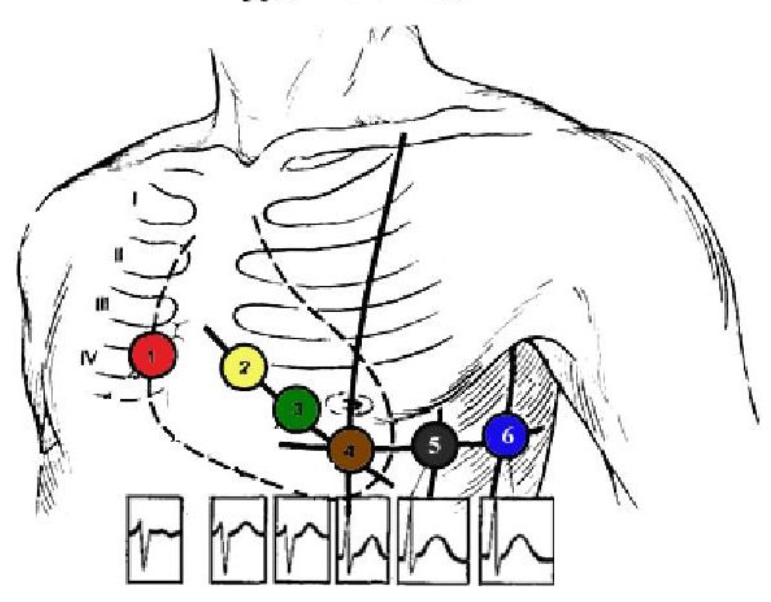
\includegraphics[scale=0.46]{resources/грудные отведения .png}
\caption{Грудные отведения.}
\label{fig:my_label}
\end{figure}

Данные отведения используются для оценки электрической активности сердца в горизонтальной плоскости. Они могут помочь выявить заболевания миокарда, такие как инфаркт миокарда и аномалии развития сердца.

\subsection{Подходы к мониторингу сердечной активности}

В настоящее время существуют различные подходы к мониторингу сердечной активности, включая:

\begin{enumerate}
    \item \textbf{Традиционные стационарные ЭКГ системы:} \\
        Высокая точность и надежность, но требуют нахождения в клинике.
    \item \textbf{Портативные ЭКГ устройства:} \\
        Легкие и удобные в использовании, но часто имеют ограниченные возможности по длительности работы и качеству связи.
    \item \textbf{Носимые устройства (например, смарт-часы с функцией ЭКГ):} \\ 
        Удобны для повседневного использования, но часто менее точны и имеют ограничения по функциональности.
\end{enumerate}

Выбор портативных ЭКГ устройств обусловлен стремлением к сочетанию высокой точности измерений с максимальной мобильностью и удобством использования, что в конечном итоге позволит обеспечить непрерывный и эффективный мониторинг сердечной активности пациента в реальном времени для своевременного реагирования на изменения состояния здоровья пациента.

\subsubsection{Вывод}

Таким образом, требуется разработать портативный аппаратный комплекс, который требует регистрации двух отведений для покрытия подавляющей области в диагностике сердечных заболеваний. Для снятия электрической активности сердца используется принцип сухих электродов.

% ========== Work made ==========
\newpage
\section{Разработка проектного решения}

Архитектура системы играет ключевую роль в обеспечении надежного и эффективного функционирования программно-аппаратного комплекса для мониторинга показателей сердца. При её проектировании было принято решение использовать принцип многослойной архитектуры. Это решение было обосновано следующими причинами:

\begin{enumerate}
    \item \textbf{Разделение обязанностей:} \
        В многоуровневой архитектуре четко определены роли компонентов, каждый из которых отвечает за определенный функционал.
    \item \textbf{Повторное использование кода:} \
        Благодаря модульной структуре многоуровневой архитектуры компоненты системы становятся более автономными и могут быть повторно использованы. Это позволяет избежать дублирования кода и обеспечивает более эффективное развитие и поддержку программного продукта.
    \item \textbf{Гибкость и масштабируемость:} \
        Многоуровневая архитектура обеспечивает гибкость и возможность модификации системы. Новые функциональные возможности могут быть легко добавлены или изменены без воздействия на другие компоненты. Кроме того, такая архитектура хорошо масштабируется при необходимости увеличения производительности или добавления новых узлов.
    \item \textbf{Улучшенная поддержка и тестирование:} \
        Четкое разграничение компонентов упрощает поддержку и тестирование системы. Каждый уровень может быть протестирован отдельно, что позволяет выявлять и исправлять ошибки на ранних стадиях разработки.
\end{enumerate}

\noindent Архитектура проекта разделена на четыре основных слоя (Рис. 3):

\begin{enumerate}
    \item Веб-приложение.
    \item Сервер для сбора, хранения и анализа данных, а также модуль для работы с базой данных.
    \item Приложение для передачи данных с ESP32 на сервер.
    \item Модуль сбора данных ЭКГ с датчиков, основанный на ESP32.
\end{enumerate}

\newpage

\begin{figure}[htbp]
    \centering
    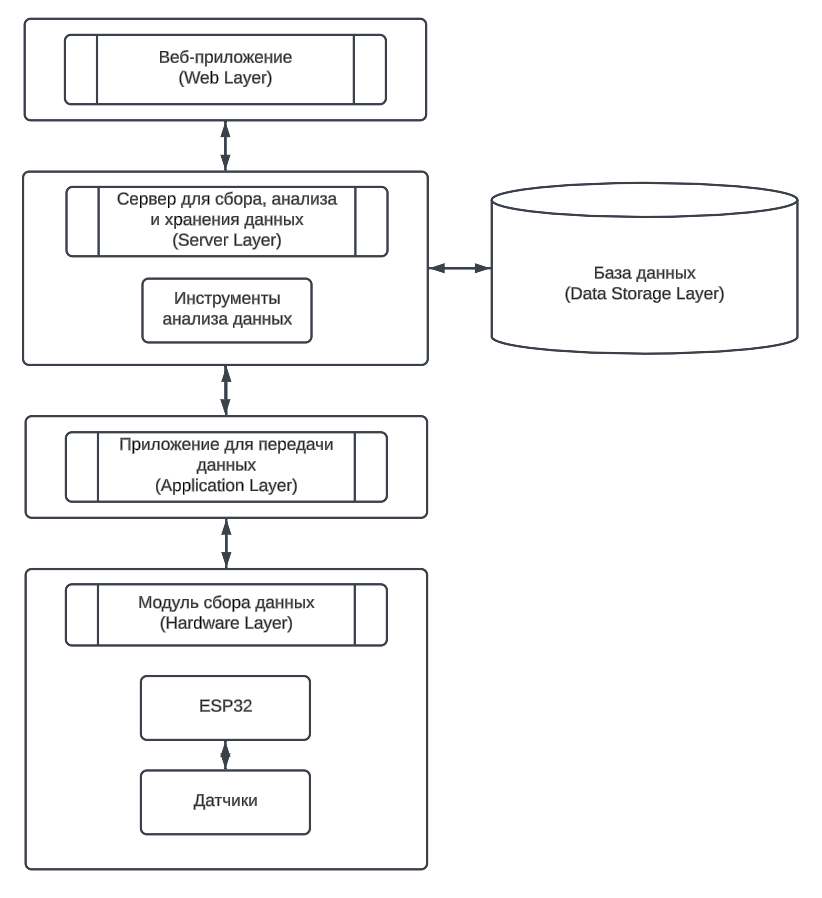
\includegraphics[scale=0.85]{resources/arch_layers.png}
    \caption{Архитектура.}
    \label{fig:my_label}
\end{figure}

Каждый слой, кроме сервера, содержит один модуль, рассмотрим каждый из них:

\begin {enumerate}
    \item \textbf{Модуль сбора данных (Hardware Layer):} \\
        Он включает в себя аппаратное обеспечение для снятия показаний ЭКГ, такое как микроконтроллер ESP32 и усилитель сигнала AD8232.
        Микроконтроллер ESP32 отвечает за считывание данных с электродов и преобразование их в цифровой формат, а также передачу в Application Layer.
        Усилитель сигнала AD8232 усиливает сигнал ЭКГ для более точного считывания.

    \item \textbf{Приложение для передачи данных (Application Layer):} \\
        Отвечает за прием, обработку и передачу данных с модуля сбора данных на сервер для анализа и хранения.
        В приложении реализована логика работы с данными, включая их форматирование, упаковку и отправку на сервер.

    \item \textbf{Сервер для сбора, анализа и хранения данных (Server Layer):} \\
        Этот слой осуществляет прием, анализ и хранение данных, полученных от приложения для передачи данных.
        В рамках сервера реализованы функциональности по обработке данных, анализу показателей сердечной активности и хранению результатов.

    \item \textbf{База данных (Data Storage Layer):} \\
        Обеспечивает долговременное хранение данных и предоставляет интерфейсы для их извлечения и манипуляций.
        Данные о показателях сердечной активности сохраняются в базе данных для последующего доступа и анализа.

    \item \textbf{Web Layer (Веб-приложение):} \\
        Этот слой предоставляет пользовательский интерфейс для взаимодействия с системой через веб-браузер. Пользователи могут просматривать данные, настраивать параметры мониторинга и получать заключения по результатам исследования ЭКГ.
\end{enumerate}

% ========== Product hardware development ==========
\newpage
\subsection{Разработка аппаратной части комплекса (Hardware Level)}

В аппаратной части проекта решающее значение имеет выбор компонентов, которые обеспечивают полноценное функционирование комплекса. Для правильного выбора компонентов требуется учитывать их стоимость, производительность, совместимость и интерфейсы коммуникации.

В этом разделе будет рассмотрен процесс выбора и обоснование использования конкретных компонентов, фокусируясь на микроконтроллере, датчиках для снятия ЭКГ и других важных устройствах для поддержки работоспособности модуля в целом.

\subsubsection{Выбор технологии передачи данных с микроконтроллера на ПК}

\noindent На текущий момент наиболее популярными технологиями являются:

\begin{itemize}
    \item Wi-Fi 
    \item Bluetooth
    \item BLE
    \item ZigBee
    \item Z-Wave
\end{itemize}

Так как ааратный комплекс должен поддерживать мониторинг на протяжении длительного времени, основным критерием отбора является энергопотребление. Высокая скорость передачи данных не требуется, т.к. максимальное количество информации, собранной за день, не может быть выше 35 МБ. 

Таким образом, наиболее подходящей технологией является BLE (Bluetooth Low Energy), главным преимуществом которой является крайне низкое потребление энергии. К примеру, средняя потребляемая мощность BLE от 0,01 Вт до 0,5 Вт, что примерно в 10 раз меньше, чем стандартная технология Bluetooth. 

\subsubsection{Выбор микроконтроллера}

При выборе микроконтроллера рассматривались следующие характеристики:

\begin{itemize}
    \item Размер платы
    \item Интегрированные модули радиосвязи, а именно BLE
    \item Наличие I2C и UART интерфейсов
    \item Энергопотребление
    \item Вычислительная мощность (кол-во ядер)
    \item Количество пинов
\end{itemize}

С учетом всех факторов, были выбраны микроконтроллеры ESP32 и ESP32-3C.
Ниже приведены основные сравнительные характеристики. 

\begin{center}
\begin{tabular}{|l|l|l|}
\hline
\textbf{}            & \textbf{ESP32} & \textbf{ESP32-3C} \\ \hline
\textbf{CPU}         & Xtensa LX6                             & RISC-V                                    \\ \hline
\textbf{Кол-во ядер} & 2                                      & 1                                         \\ \hline
\textbf{Пины GPIO}        & 34                                     & 22                                        \\ \hline
\textbf{Потребление} & До 325 мА                              & До 240 мА                                 \\ \hline
\textbf{Размеры}     & 31 x 18 x 3.0 мм                       & 24 x 16 x 3.1 мм                          \\ \hline
\end{tabular}
\end{center}

По итогу решено использовать микроконтроллер ESP32-3C поскольку он обладает меньшими размерами и более низким энергопотреблением, однако придется столкнуться с проблемами производительности поскольку выбранный микроконтроллер имеет одно ядро и нельзя будет отправлять полученные данные в фоновом режиме на втором ядре.

\subsubsection{Выбор датчика для снятия ЭКГ}

При выборе модели датчика сердечного ритма были определены следующие критерии, которым он должен соответствовать: 

\begin{enumerate}
    \item Датчик должен поддерживать считывание на частоте в 100 Гц
    \item Датчик не должен иметь больших размеров
    \item Измерения датчика должны быть разборчивыми
    \item Цена датчика должна быть бюджетной
\end{enumerate}

После проведения анализа было решено остановиться на следующих датчиках: 

\begin{itemize}
    \item AD8232
    \item CJMCU-333
\end{itemize}

Далее проходил этап их сравнения на тестовом стенде.

Чтобы свести к минимуму влияние внешних факторов на показания датчиков было решено разработать тестирующий стенд.
Основным питающим элементом была литиевая батарея, чтобы избежать зашумления сигнала, которое может возникнуть при питании от сети.

Приведем описание для датчиков, которые были главными претендентами на выбор.

\subsubsection{Тестирование CJMCU-333}

CJMCU333 — маломощный прецизионный инструментальный усилитель. Датчик имеет универсальную конструкцию с тремя операционными усилителями, небольшой размер и малое энергопотребление. Один внешний резистор устанавливает любой коэффициент усиления от 1 до 1000 (Рис. 4).

\begin{figure}[htbp]
\centering
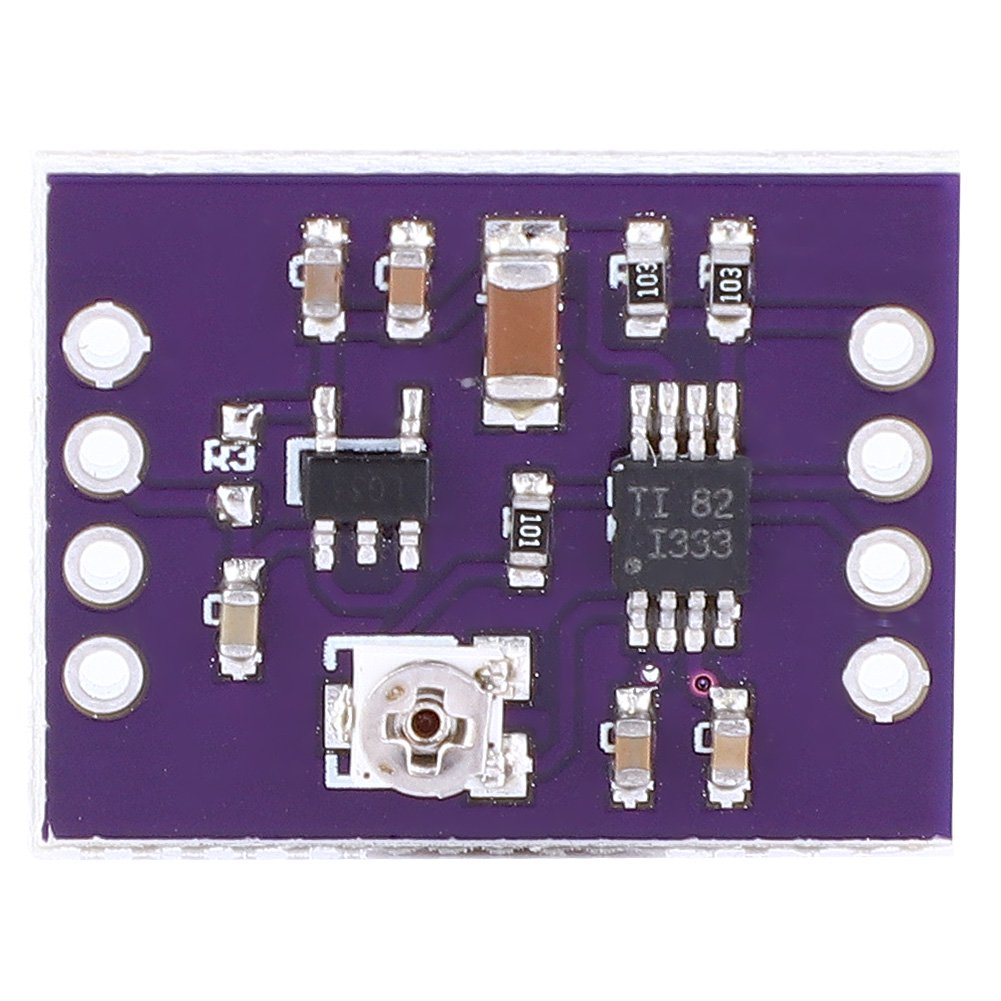
\includegraphics[scale=0.15]{resources/cjmcu333/cjmcu-333.png}
\caption{CJMCU-333}
\label{fig:my_label}
\end{figure}

После калибровки и тестирования, ЭКГ выглядело следующим образом (Рис. 5, 6).

\begin{figure}[htbp]
\centering
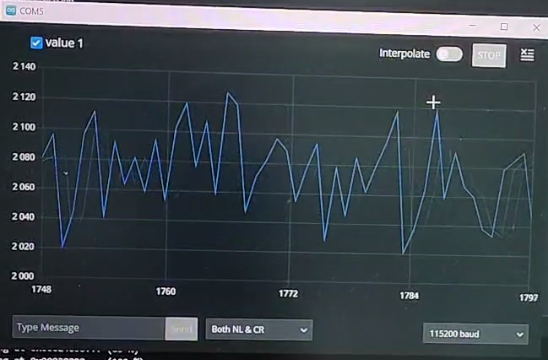
\includegraphics[scale=0.6]{resources/cjmcu333/1.png}
\caption{CJMCU-333 ЭКГ Пример-1.}
\label{fig:my_label}
\end{figure}

\begin{figure}[htbp]
\centering
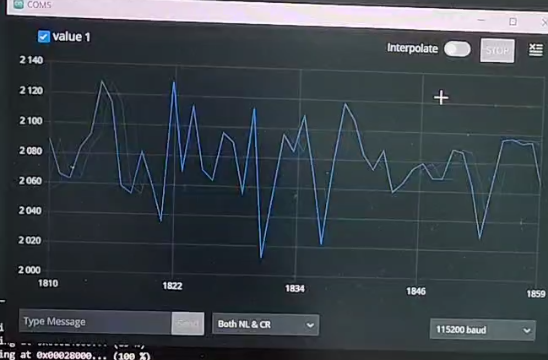
\includegraphics[scale=0.6]{resources/cjmcu333/2.png}
\caption{CJMCU-333 ЭКГ Пример-2.}
\label{fig:my_label}
\end{figure}

\newpage

После проведения немалого количества трудоемких настроек датчика были результаты, который можно видеть в прикрепленных картинках.
По графикам невозможно отследить периодичность. Кривая имеет большое количество артефактов и шума. Разобрать данную ЭКГ-кардиограмму не представляется возможным. Результаты тестирования были неудовлетворительными, поэтому данный датчик применяться в проекте не будет.

\subsubsection{Тестирование AD8232}

AD8232 — это интегрированный блок формирования сигнала для ЭКГ и других приложений измерения биопотенциала. Он предназначен для извлечения, усиления и фильтрации слабых сигналов биопотенциала в условиях шумов, например, создаваемых движением или удаленным размещением электродов (Рис. 7).

\begin{figure}[htbp]
\centering
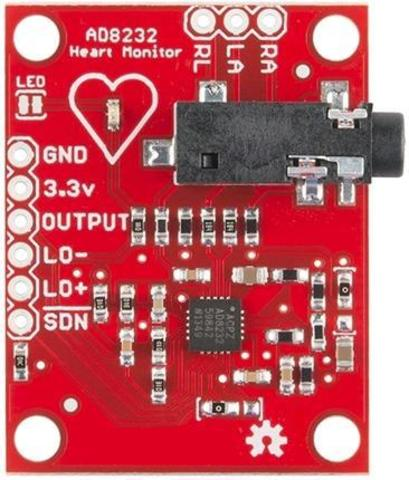
\includegraphics[scale=1.4, angle=90]{resources/ad8232/ad8232.png}
\caption{AD8232}
\label{fig:my_label}
\end{figure}

При тестировании график ЭКГ выглядел следующим образом (Рис. 8).

\begin{figure}[htbp]
\centering
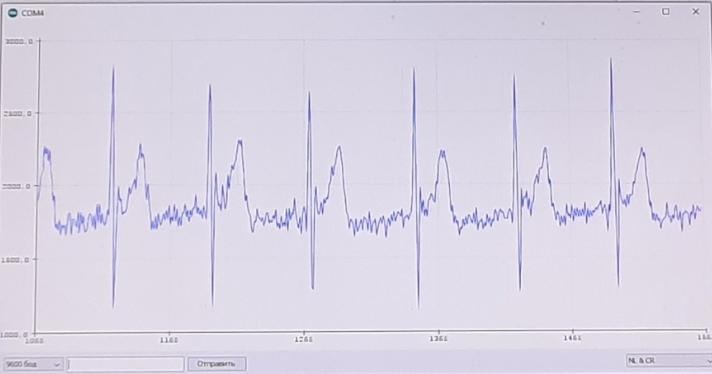
\includegraphics[scale=0.5]{resources/ad8232/1е-отведение.jpg}
\caption{График AD8232 1-ое отведение.}
\label{fig:my_label}
\end{figure}

По результатам первых тестов можно заметить, что показатели получаются довольно точными и чистыми. Кривая имеет выраженную периодичность, а также точно прослеживаются зубцы. В качестве эксперимента было проведено считывание ЭКГ по второму отведению (Рис. 9).

\begin{figure}[htbp]
\centering
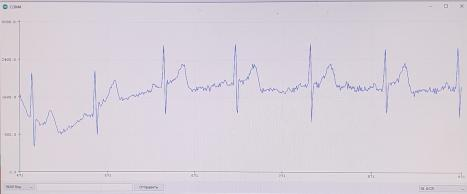
\includegraphics[scale=0.8]{resources/ad8232/2е-отведение.jpg}
\caption{График AD8232 2-ое отведение.}
\label{fig:my_label}
\end{figure}

А также по значениям первого и второго отведений было вычислено третье отведение с последующем отображением значений в виде графика (Рис. 9).

\begin{figure}[htbp]
\centering
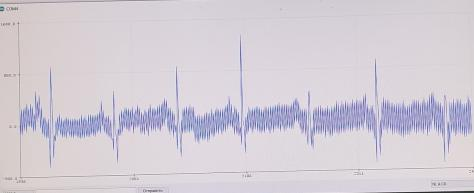
\includegraphics[scale=0.8]{resources/ad8232/3е-отведение.jpg}
\caption{График AD8232 3-ое отведение.}
\label{fig:my_label}
\end{figure}

Таким образом, из всех протестированных датчиков был выбран именно AD8232, поскольку только с его помощью удалось достичь таких качественных результатов.

\subsubsection{Разработка модели}

При разработке модуля необходимо учитывать возможность его размещения на спортивной майке, а значит он должен иметь относительно небольшие размеры и маленький вес. Так как модуль необходимо будет заряжать и отправлять с него данные на сервер было принято решение разбить его на два подмодуля. Так, в первом подмодуле будут располагаться электроды и датчики считывания ЭКГ, а во втором то, что необходимо для сохранения, обработки и передачи полученных данных.

\par\textbf{Подмодуль ЭКГ}

Экспериментальным путем было выяснено, что наиболее подходящей моделью датчика сердечного ритма является AD8232. Так как нам требуется считывать два типа отведений минимум, а каждый датчик может считывать максимум один, нам потребуется использовать их сразу два. Примитивная схема данного подмодуля выглядит следующим образом (Рис. 11).

\begin{figure}[htbp]
\centering
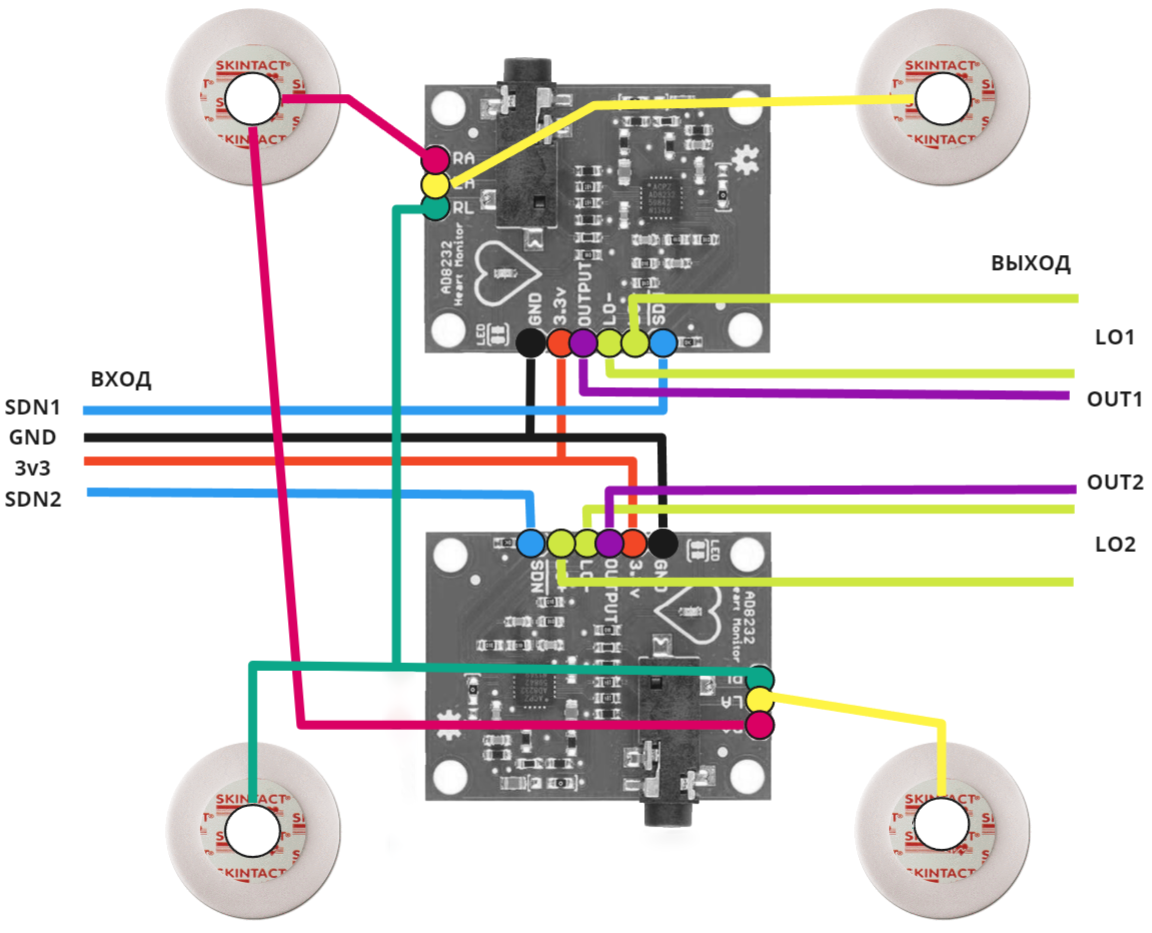
\includegraphics[scale=0.5]{resources/sub1.png}
\caption{Подмодуль ЭКГ.}
\label{fig:my_label}
\end{figure}

На вход в данный подмодуль поступает четыре провода:

\begin{itemize}
    \item SDN1
    \item GND
    \item 3v3
    \item SDN2
\end{itemize}

Провода типа SDN отвечают за перевод подключенного к ним датчика в энергосберегающий режим. GND и 3v3 отвечают за питание датчиков.

На выход идет шесть проводов: 

\begin{itemize}
    \item два провода типа LO1
    \item два провода типа LO2
    \item OUT1
    \item OUT2
\end{itemize}

Провода типа LO передают сигнал о том, что электроды подключены к датчику и с них считывается сигнал. Провод OUT1 отправляет значение ЭКГ по первому типу отведения, OUT2 по второму.

\par\textbf{Подмодуль с микроконтроллером}

Основная задача данного подмодуля является считывание данных с датчиков ЭКГ, промежуточное хранение и их последующая отправка. Для сохранения большого объема информации на определенное время требуется внешний накопитель. Так как модуль является автономным, для него требуется батарея с возможностью зарядки.

Таким образом, минимальный набор требуемых компонентов выглядит следующим образом:

\begin{itemize}
    \item ESP32-3C
    \item Преобразователь напряжение в 3В
    \item Модуль с SD-картой
    \item Модуль для зарядного устройства
    \item Литий-ионная батарея
    \item Магнитный коннектор
\end{itemize}

Исходя из этого, была разработана примитивная схема данного подмодуля (Рис. 12).
\newpage

\begin{figure}[htbp]
\centering
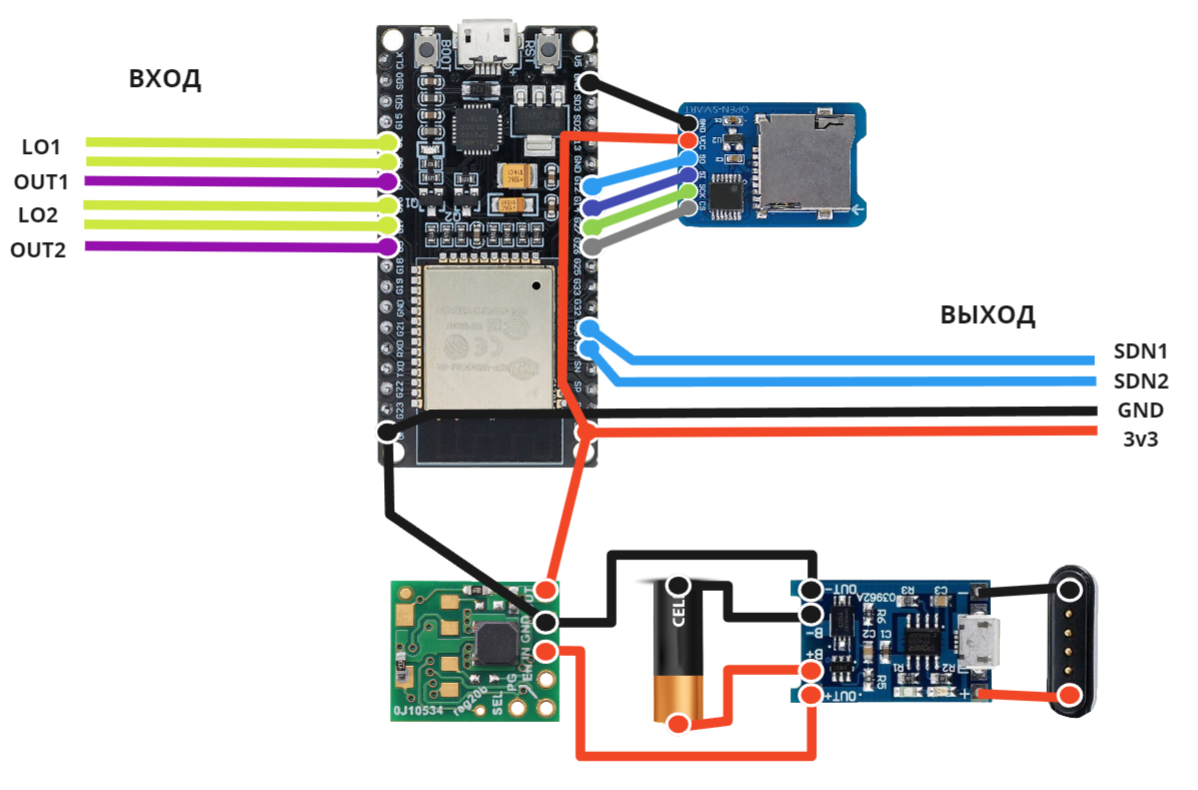
\includegraphics[scale=0.48]{resources/2.png}
\caption{Подмодуль с микроконтроллером.}
\label{fig:my_label}
\end{figure}

Входные и выходные провода соединятся с подмодулем ЭКГ, поэтому ознакомится с назначением каждого провода можно в вышеупомянутом разделе.

\par \noindent \textbf{3D модель}

Для проектирования первой тестовой модели был использован инструмент Tinkercad из-за простоты использования для создания примитивных объектов. Полученная модель была распечатана на 3D принтере.

% ========== Product software development ==========
\newpage
\subsection{Разработка программной части комплекса (Software level)}

В программной части комплекса необходимо было выбрать правильные технологии, инструменты и методы разработки.

В данном разделе будет рассмотрен процесс выбора технологий и методов разработки, обоснование принятых решений и анализ их влияния на функциональность и эффективность всего комплекса мониторинга, а также определение функциональных и нефункциональных требований.

\subsubsection{Разработка требований к программной части комплекса (ПЧК)}

Требования к программной части комплекса можно разделить на функциональные и нефункциональные.

\noindent
\textbf{Функциональные требования:}

\begin{enumerate}
    \item \textbf{Сбор данных ЭКГ:} \\
        ПЧК должен уметь собирать данные ЭКГ с помощью модуля ESP32 и AD8232.
    \item \textbf{Передача данных:} \\
        Данные ЭКГ должны передаваться от модуля на сервер в реальном времени.
    \item \textbf{Анализ данных:} \\
        Сервер должен анализировать поступающие данные, выявлять аномалии и предупреждать пользователя.
    \item \textbf{Хранение данных:} \\
        Данные должны сохраняться в базе данных для последующего анализа и отчетности.
    \item \textbf{Пользовательский интерфейс:} \\
        ПЧК должен иметь удобный пользовательский интерфейс для просмотра текущих и исторических данных ЭКГ, а также для получения заключений по показаниям ЭКГ.
    \item \textbf{Отображение данных в реальном времени:} \\
        Пользователям должна быть предоставлена
        возможность мониторинга показаний ЭКГ в реальном времени через веб-интерфейс.
\end{enumerate}

\noindent
\textbf{Нефункциональные требования:}

\begin{enumerate}
    \item \textbf{Отказоустойчивость:} \\
        Приложение должно быть устойчивым к сбоям и обеспечивать непрерывную работу в течение длительного времени.
    \item \textbf{Безопасность данных:} \\
        Все данные, передаваемые между компонентами системы, должны быть защищены с помощью соответствующих механизмов шифрования и аутентификации.
    \item \textbf{Производительность:} \\
        Приложение должно обеспечивать высокую производительность при передаче и обработке данных, чтобы минимизировать задержки и обеспечить оперативную реакцию на изменения состояния пациента.
    \item \textbf{Масштабируемость:} \\
        Система должна быть способна масштабироваться в зависимости от количества пользователей и объема данных, обрабатываемых ежедневно.
    \item \textbf{Простота использования:} \\
        Веб-интерфейс должен быть интуитивно понятным и легким в использовании даже для неопытных пользователей.
\end{enumerate}

% ========== Application layer ==========
\subsubsection{Разработка программной части для модуля сбора данных на базе ESP32}

\par \noindent \textbf{Выбор фреймворка}

Для разработки программного обеспечения на ESP32 был выбран Arduino Framework в связке с PlatformIO благодаря простоте и удобству использования. Arduino Framework предоставляет все необходимые инструменты для написания, компиляции и загрузки кода на микроконтроллер. Его поддержка широкого спектра библиотек и большая пользовательская база делают решение возникающих проблем более легким.

\par \noindent \textbf{Архитектура}

При проектировании программного обеспечения использовался модульный подход, что позволяет изолировать различные функциональные компоненты системы. Это упрощает разработку, отладку и сопровождение кода, а также способствует повторному использованию и легкости расширения.

В системе используется паттерн Singleton, что позволяет гарантировать, что каждый модуль имеет только одну глобальную точку доступа. Это особенно важно для модулей, которые управляют аппаратными ресурсами, такими как SD-карта или BLE-сервисы. Singleton паттерн обеспечивает уникальность экземпляра и глобальный доступ к нему, что упрощает управление состоянием и ресурсами.

\par \noindent \textbf{Структура программного кода на ESP32}

Работа с модулями организована путем разделения на заголовочные файлы (.h) и файлы реализации (.cpp). Заголовочные файлы содержат объявления функций и классов, обеспечивая интерфейс между модулями, тогда как файлы реализации содержат конкретную реализацию этих функций.

\par \noindent \textbf{Модули и точка входа}

\begin{enumerate}
    \item \textbf{BLE Service Handler Module} \\
        Обрабатывает взаимодействие через Bluetooth Low Energy (BLE). Включает функции для настройки и обработки BLE-соединений.
    \item \textbf{Configuration Helper Module} \\
        Содержит параметры конфигурации, такие как настройки сети и параметры подключения. Обеспечивает централизованное управление конфигурациями.
    \item \textbf{Data Package Module} \\
        Осуществляет упаковку и распаковку данных для передачи. Включает структуры данных и функции для их обработки.
    \item \textbf{SPI Flash Module} \\
        Управляет взаимодействием с SPI Flash памятью. Содержит функции для чтения и записи данных во флеш-память.
    \item \textbf{Main Module(Основная точка входа в программу)} \\
        Отвечает за инициализацию системы и подключение модулей. Также содержит основной цикл работы, в котором происходит вызов функций других модулей. Также в этом модуле происходит считывание сигнала ЭКГ с модулей AD8232, используя интерфейсы I2C.
\end{enumerate}

\par \noindent \textbf{Основная логика работы программы}

Основная логика работы, инициализация и управление модулями содержится в Main Module программы. Ключевыми элементами данного модуля являются две основные функции Arduino Framework, а именно:

\begin{itemize}
    \item \textbf{setup():} Инициализация системы и подключение модулей.
    \item \textbf{loop():} Основной цикл работы, в котором происходит вызов функций других модулей.
\end{itemize}

Рассмотрим основную логику работы этих функций:

\par \noindent \textbf{setup():}

\begin{enumerate}
    \item Инициализация серийного порта для вывода отладочной информации.
    \item Настройка BLE-сервиса с помощью вызова соответствующих функций из BLE Service Handler.
    \item Инициализация и настройка портов для работы с AD8232.
    \item Загрузка конфигурации из SPI Flash памяти.
\end{enumerate}

\par \noindent \textbf{loop():}

\begin{enumerate}
    \item Циклический опрос состояния системы.
    \item Сбор данных с сенсоров и их обработка.
    \item Упаковка данных с помощью Data Package Module.
    \item Передача данных через BLE на сервер.
    \item Управление состояниями системы и обработка событий, таких как потеря соединения или ошибки передачи данных. (В данном случае данные сохраняются на SD карту)
\end{enumerate}

\par \noindent \textbf{Тестирование}

В ходе разработки проекта возникли ограничения в виде отсутствия собранного тестирующего стенда, что затруднило проведение автоматизированного традиционного тестирования.

На данный момент применяется тестирование модуля только в области форматирования и проверки стиля кода, который на него загружается, что в конечном итоге все равно способствует повышению его читаемости и качества.

% ========== Application layer ==========
\subsubsection{Приложение для передачи данных (Application Layer)}

Electron-приложение служит посредником для передачи данных ЭКГ с устройства ESP32 на сервер. Для обеспечения безопасности и функциональности приложения были выделен набор наиболее важных сценарев использования.

\par \noindent \textbf{Сценарии использования}

\begin{itemize}
    \item \textbf{Аутентификация и авторизация:} \\
        \begin{enumerate}
            \item Пользователь открывает Electron приложение и вводит свои учетные данные (логин и пароль).
            \item Приложение отправляет данные на сервер для аутентификации.
            \item В случае успешной аутентификации пользователь получает доступ к функционалу приложения.
            \item Пользователь может выйти из системы, закрыв Electron приложение или используя соответствующую функцию в интерфейсе приложения.
            \item После выхода из системы пользователь теряет доступ к функционалу приложения до следующего входа.
        \end{enumerate}
    \item \textbf{Отправка данных ЭКГ на анализ c ESP32 на сервер:} \\
        \begin{enumerate}
            \item Пользователь может отправлять данные ЭКГ на сервер для анализа и получения дополнительной информации о своем состоянии здоровья с помощью технологии BLE.
        \end{enumerate}
    \item \textbf{Просмотр метаданных:} \\
        \begin{enumerate}
            \item Пользователь может видеть общее количество отправленных пакетов.
            \item Пользователь может просматривать информацию о качестве подключения.
        \end{enumerate}
\end{itemize}

Проектированием и разработкой этого модуля занимался студент группы 382006-2 Юнин Даниил Дмитриевич.

% ========== Server ==========
\subsubsection{Сервер для сбора, анализа и хранения данных (Server Layer)}

\par \noindent \textbf{Выбор фреймворка и языка}

Python вместе с Flask был выбран в качестве основного фреймворка для разработки серверной части веб-приложения по нескольким причинам:

\begin{enumerate}
    \item \textbf{Легковесность и Гибкость:} \\
        Flask отличается простотой и легковесностью в использовании, что делает его идеальным выбором для разработки небольших и средних проектов. При этом, он обладает достаточной гибкостью, чтобы удовлетворить потребности различных задач.
    \item \textbf{Простота Создания RESTful API:} \\
        Flask предоставляет все необходимые инструменты для создания RESTful API, что позволяет легко интегрировать сервер с различными компонентами системы. Это критически важно для проекта, где требуется эффективное взаимодействие с базой данных и клиентскими приложениями.
    \item \textbf{Широкая Поддержка Библиотек:} \\
        Язык программирования Python обладает богатой экосистемой библиотек, что делает его идеальным выбором для разработки веб-приложений. Python предоставляет широкие возможности для анализа данных, что идеально подходит для обработки медицинских данных.
\end{enumerate}

\par \noindent \textbf{Архитектура}

В разработке серверной части веб-приложения использован принцип архитектуры, основанный на модели MVC (Model-View-Controller), дополненный использованием REST API для взаимодействия с клиентской стороной, написанной на Vue.js.

На серверной стороне, основные компоненты архитектуры включают в себя:

\begin{itemize}
    \item \textbf{Модель (Model):} \\
        Представлена моделями данных и логикой взаимодействия с базой данных, реализованными с использованием ORM (объектно-реляционного отображения). Данные хранятся и обрабатываются на сервере, что обеспечивает централизованное хранение и управление информацией.
    \item \textbf{Представление (View):} \\
        Фронтенд, написанный на Vue.js, действует как "представление" и отображает данные, полученные через REST API от сервера. Фронтенд обеспечивает пользовательский интерфейс для взаимодействия с приложением и представляет пользовательский опыт.
    \item \textbf{Контроллер (Controller):} \\
        Контроллеры, представленные в виде маршрутов в API, обрабатывают HTTP-запросы от клиента и возвращают соответствующие данные. Они являются посредниками между моделью и представлением, обеспечивая передачу данных между ними и управление бизнес-логикой приложения.
\end{itemize}

Помимо этого, в архитектуре также будет интегрирован модуль взаимодействия с приложением на Electron. Этот модуль будет отвечать за получение данных ЭКГ для дальнейшей обработки на сервере, а также за отображение ЭКГ и заключений на клиентской стороне приложения. Таким образом, функциональность приложения расширяется, обеспечивая его более широкий спектр использования.

Данный подход обеспечивает четкое разделение бизнес-логики, представления данных и управления запросами на отдельные компоненты, что делает приложение более модульным, легко сопровождаемым и масштабируемым.

\par \noindent \textbf{Структура сервера}

\par \noindent \textbf{Модуль ORM и Работа с Базой Данных (ORM and Database Handling)}
\begin{itemize}
    \item \textbf{Описание}: Модуль отвечает за взаимодействие с базой данных с помощью объектно-реляционного отображения и выполнения SQL-запросов.
    \item \textbf{Назначение}:
    \begin{itemize}
        \item Определение моделей данных.
        \item Управление транзакциями базы данных.
        \item Обеспечение абстракции для работы с реляционными данными.
        \item Подключение к базе данных.
        \item Управление схемой базы данных и инициализация данных.
    \end{itemize}
    \item \textbf{Компоненты}:
    \begin{itemize}
        \item Модели данных.
        \item Конфигурация базы данных.
        \item Скрипты инициализации базы данных.
        \item Сессии для взаимодействия с базой данных.
    \end{itemize}
\end{itemize}

\par \noindent \textbf{Модуль Роутинга (Routing)}
\begin{itemize}
    \item \textbf{Описание}: Модуль управляет маршрутами и эндпоинтами API.
    \item \textbf{Назначение}:
    \begin{itemize}
        \item Определение URL маршрутов.
        \item Обработка входящих HTTP-запросов.
        \item Связывание запросов с соответствующими функциями контроллеров.
    \end{itemize}
    \item \textbf{Компоненты}:
    \begin{itemize}
        \item Маршруты для аутентификации.
        \item Маршруты для работы с веб-приложением.
        \item Маршруты для поддержания взаимодействия с модулем Electron.
    \end{itemize}
\end{itemize}

\par \noindent \textbf{Модуль ИИ для Анализа Данных (AI Data Analysis)}
\begin{itemize}
    \item \textbf{Описание}: Модуль использует алгоритмы машинного обучения и другие методы искусственного интеллекта для анализа данных ЭКГ.
    \item \textbf{Назначение}:
    \begin{itemize}
        \item Предобработка данных ЭКГ.
        \item Анализ и классификация данных ЭКГ.
        \item Генерация заключений на основе анализа.
    \end{itemize}
    \item \textbf{Компоненты}:
    \begin{itemize}
        \item Алгоритмы машинного обучения.
        \item Модели для анализа данных.
        \item Методы предсказания и оценки.
    \end{itemize}
\end{itemize}

\par \noindent \textbf{Модуль Взаимодействия с Electron (Electron Integration)}
\begin{itemize}
    \item \textbf{Описание}: Модуль обеспечивает интеграцию с десктопным приложением, написанным на Electron.
    \item \textbf{Назначение}:
    \begin{itemize}
        \item Получение данных ЭКГ от десктопного приложения.
    \end{itemize}
    \item \textbf{Компоненты}:
    \begin{itemize}
        \item API для взаимодействия с Electron.
        \item Логика обработки входящих данных.
    \end{itemize}
\end{itemize}

\par \noindent \textbf{Модуль Аутентификации и Авторизации (Authentication and Authorization)}
\begin{itemize}
    \item \textbf{Описание}: Модуль управляет регистрацией, входом и выходом пользователей, а также контролем доступа.
    \item \textbf{Назначение}:
    \begin{itemize}
        \item Обработка регистрации и аутентификации пользователей.
        \item Управление сессиями и токенами.
        \item Обеспечение безопасности доступа к API.
    \end{itemize}
    \item \textbf{Компоненты}:
    \begin{itemize}
        \item Методы регистрации и входа пользователей.
        \item Управление JWT токенами.
        \item Политики доступа и проверки прав пользователей.
    \end{itemize}
\end{itemize}

\par \noindent \textbf{Модуль Логирования и Мониторинга (Logging and Monitoring)}
\begin{itemize}
    \item \textbf{Описание}: Модуль отвечает за запись логов и мониторинг состояния системы.
    \item \textbf{Назначение}:
    \begin{itemize}
        \item Логирование ошибок и событий.
        \item Мониторинг производительности и состояния системы.
    \end{itemize}
    \item \textbf{Компоненты}:
    \begin{itemize}
        \item Конфигурация логирования.
        \item Методы мониторинга.
    \end{itemize}
\end{itemize}

\par \noindent \textbf{Модуль Тестирования (Testing)}
\begin{itemize}
    \item \textbf{Описание}: Модуль обеспечивает тестирование всех компонентов сервера.
    \item \textbf{Назначение}:
    \begin{itemize}
        \item Написание и выполнение тестов для проверки функциональности.
        \item Обеспечение качества кода и предотвращение ошибок.
    \end{itemize}
    \item \textbf{Компоненты}:
    \begin{itemize}
        \item Тесты для маршрутов и API.
        \item Тесты для взаимодействия с базой данных.
        \item Тесты для модулей ИИ и анализа данных.
    \end{itemize}
\end{itemize}

\par \noindent \textbf{Основная логика работы программы}

\par \noindent \textbf{Инициализация и настройка приложения}
\begin{enumerate}
    \item При запуске приложения инициализируется объект Flask.
    \item Устанавливается соединение с базой данных.
    \item Настраивается JWT для безопасной аутентификации пользователей.
\end{enumerate}

\par \noindent \textbf{Обработка запросов}
\begin{enumerate}
    \item При поступлении запроса на сервер, Flask маршрутизирует его к соответствующему обработчику.
    \item Обработчики маршрутов выполняют необходимые операции, включая обработку запросов аутентификации, доступа к данным, выполнение бизнес-логики и т.д.
\end{enumerate}

\par \noindent \textbf{Аутентификация и авторизация}
\begin{enumerate}
    \item При получении запроса, требующего аутентификации, сервер проверяет наличие и валидность JWT в заголовке запроса.
    \item Если токен действителен, пользователь получает доступ к запрашиваемым ресурсам или операциям.
\end{enumerate}

\par \noindent \textbf{Взаимодействие с данными}
\begin{enumerate}
    \item При выполнении запросов на получение, создание, обновление или удаление данных, сервер взаимодействует с базой данных через модели и ORM SQLAlchemy.
    \item Данные могут быть переданы обратно клиенту в виде JSON или другого формата в зависимости от запроса.
\end{enumerate}

\par \noindent \textbf{Работа с ИИ}
\begin{enumerate}
    \item При получении данных ЭКГ от клиента или других источников, сервер обрабатывает их с использованием алгоритмов машинного обучения и анализа данных.
    \item Результаты анализа, включая диагностику и заключения, могут быть отправлены обратно клиенту для отображения и дальнейшего использования.
\end{enumerate}

Проектированием и разработкой этой части модуля занимался студент группы 382006-2 Юнин Даниил Дмитриевич.

\par \noindent \textbf{Тестирование}
\begin{enumerate}
    \item При разработке нового функционала, сервер проходит тестирование вручную с помощью разработанных модульных тестов.
    \item Тесты включают в себя проверку основных сценариев использования, а также тестирование работы с данными и взаимодействия с клиентами.
\end{enumerate}

\par \noindent \textbf{Использование Docker для контейнеризации приложения}

Поскольку сервер будет запущен на специально выделенной временной удаленной машине, контейнеризация необходима, что обеспечить независимость от окружения, что упрощает развертывание и масштабирование системы. Docker гарантирует, что приложение будет работать одинаково на всех платформах, предоставляя единое окружение для разработки, тестирования и производства.

% ========== Data storage level ==========
\subsubsection{База данных (Data Storage Layer)}

\par \noindent \textbf{Выбор СУБД}


При принятии решения о выборе базы данных для проекта важно провести тщательный анализ доступных вариантов, учитывая их особенности, преимущества и недостатки. На рассмотрении находились следующие варианты:


\begin{itemize}
    \item \textbf{SQLite:} легковесная база данных, хранящаяся в виде одного файла, что обеспечивает простоту использования и удобство встроенного хранения данных для приложений с небольшим объемом информации.
    \item \textbf{MySQL:} широко известная реляционная база данных с открытым исходным кодом, которая обладает высокой производительностью и надежностью, что делает ее предпочтительным выбором для развертывания крупных и высоконагруженных систем.
    \item \textbf{MongoDB:} NoSQL база данных, ориентированная на хранение документов, что обеспечивает гибкость в работе с неструктурированными данными и удобство масштабирования.
    \item \textbf{Redis:} ин-memory база данных, специализирующаяся на хранении данных в оперативной памяти, обеспечивающая высокую скорость доступа к данным и широкое применение для кэширования и хранения временных данных.
\end{itemize}

По итогу, было решено использовать PostgreSQL из-за его надежности, расширяемости, а также доступности.
Кроме того, PostgreSQL активно развивается сообществом и имеет обширную документацию,
что делает его привлекательным выбором для учебных проектов.

\par \noindent \textbf{Проектирование структуры БД}

\begin{enumerate}
    \item \textbf{Создание схемы базы данных:}
        \begin{itemize}
            \item В ходе проектирования было определено три основных сущности: пользователи
                данные ЭКГ и аутентификационные данные.
            \item Для каждой сущности была разработана соответствующая таблица в базе данных,
                представляющая собой логическую структуру для хранения данных.
        \end{itemize}
    \item \textbf{Определение полей и их типов:}
        \begin{itemize}
            \item Каждая таблица содержит набор полей, определяющих характеристики сущности.
            \item Типы данных для полей выбирались с учетом требований к хранению и обработке информации.
        \end{itemize}
    \item \textbf{Определение отношений между таблицами:}
        \begin{itemize}
            \item Для связывания данных между таблицами были определены внешние ключи и отношения.
            \item Например, таблица аутентификационных данных имеет внешний ключ, связывающий ее с таблицей пользователей.
        \end{itemize}
\end{enumerate}

\par \noindent \textbf{Использование Docker для контейнеризации приложения}

Для базы данных PostgreSQL также был создан собственный сервис и контейнер для гарантирования работоспособности приложения на всех платформах.


% ========== Web layer ==========
\subsubsection{Web Layer (Веб-приложение)}

Web-приложение является основным источником для изучения и рассмотрения пользователем своих данных ЭКГ. Оно реализовано как одностраничное приложение (SPA), предоставляющее пользователю удобный интерфейс для взаимодействия с данными. Перед началом проектирования были выделены основные сценарии использования веб-приложения. 

\par \noindent \textbf{Сценарии использования}

\begin{enumerate}
    \item \textbf{Авторизация и аутентификация:}
    \begin{itemize}
        \item Пользователи могут войти в систему, предоставив свои учетные данные.
        \item После успешной аутентификации пользователи получают доступ к функционалу приложения.
    \end{itemize}

    \item \textbf{Заполнение профиля:}
    \begin{itemize}
        \item Пользователи имеют возможность добавлять и изменять свои личные данные в своем профиле.
        \item Обновленные данные сохраняются на сервере для последующего использования.
    \end{itemize}

    \item \textbf{Отображение графиков данных ЭКГ:}
    \begin{itemize}
        \item Пользователи могут запрашивать просмотр графиков данных ЭКГ, полученных от Electron приложения.
        \item Графики отображаются в интерфейсе приложения для удобного изучения пользователем своих данных.
    \end{itemize}

    \item \textbf{Отображение показаний здоровья и рекомендаций:}
    \begin{itemize}
        \item Пользователям предоставляется информация о их текущем состоянии здоровья, основанная на данных ЭКГ и других медицинских параметрах.
        \item Кроме того, пользователи могут получать рекомендации по улучшению своего здоровья на основе анализа предоставленных данных.
    \end{itemize}
\end{enumerate}

Проектированием и разработкой этого модуля занимался студент группы 382006-2 Юнин Даниил Дмитриевич.

% ========== Conclusion ==========
\newpage
\section{Практическая апробация и внедрение}

% ========== References ==========
\newpage
\section{Список литературы}


% ========== Additional 
\newpage
\section{Приложение}

\end{spacing}
\end{document}



